\documentclass[10pt,a4paper, margin=1in]{article}
\usepackage{fullpage}
\usepackage{amsfonts, amsmath, pifont}
\usepackage{amsthm}
\usepackage{graphicx}
\usepackage{float}
\usepackage{mathtools} 
\usepackage{extarrows}
\usepackage{bigints}

\usepackage{tkz-euclide}
\usepackage{tikz}
\usepackage{pgfplots}
\pgfplotsset{compat=1.13}

\usepackage{geometry}
 \geometry{
 a4paper,
 total={210mm,297mm},
 left=10mm,
 right=10mm,
 top=10mm,
 bottom=10mm,
 }
 % Write both of your names here. Fill exxxxxxx with your ceng mail address.
 \author{
  Adıgüzel, Gürhan İlhan\\
  \texttt{e2448025@ceng.metu.edu.tr}
  \and
  İçen, Anıl\\
  \texttt{e2448488@ceng.metu.edu.tr}
}

\title{CENG 384 - Signals and Systems for Computer Engineers \\
Spring 2023 \\
Homework 3}
\begin{document}
\maketitle

\begin{filecontents}{q4a_1.dat}
 n   a_k
 -2  0.5
 -1  1.11
 0   1
 1   1.11
 2   0.5
\end{filecontents}

\begin{filecontents}{q4a_2.dat}
 n    a_k
 -2   -45
 -1   26.57
 0    1
 1    -26.57
 2    45
\end{filecontents}

\begin{filecontents}{q6a_1.dat}
 n   xn
 0   1
 1  -0.5
 2   0
 3   -0.5
\end{filecontents}

\begin{filecontents}{q6a_2.dat}
 n   a_k
 -3  0.5
 -2  0
 -1  0.5
 0   1
 1   0.5
 2   0
 3   0.5
 4   1
\end{filecontents}

\begin{filecontents}{q6a_3.dat}
 n   a_k
 -3  180
 -2  0
 -1  180
 0   0
 1   180
 2   0
 3   180
 4   0
\end{filecontents}


\begin{filecontents}{q6b_1.dat}
 n   xn
 -3  0.559
 -2  0.25
 -1  0.559
 0   0.75
 1   0.559
 2   0.25
 3   0.559
 4   0.75
\end{filecontents}


\begin{filecontents}{q6b_2.dat}
 n   xn
 -3  -153
 -2  0
 -1  153
 0   0
 1   0153
 2   0
 3   153
 4   0
\end{filecontents}

\noindent\rule{19cm}{1.2pt}

\begin{enumerate}

\item %write the solution of q1
    \\\\Firstly, we know that $\int_{-\infty}^{\infty}x(t)dt$ is finite valued and periodic only if $a_{0}$ = 0.
    \\\\Then,
    \\\\ $x(t) = \Sigma_{k=-\infty}^{\infty}a_{k}e^{jkw_{0}t} $
    \\\\t $\longrightarrow s$
    \\\\ $x(s) = \Sigma_{k=-\infty}^{\infty}a_{k}e^{jkw_{0}s}$
    \\\\ $\int_{-\infty}^{t}x(s)ds =\Sigma_{k=-\infty}^{\infty}a_{k}\int_{-\infty}^{\infty}e^{jkw_{0}s}ds$ 
    \\\\  $\int_{-\infty}^{t}x(s)ds =\Sigma_{k=-\infty}^{\infty}a_{k} \dfrac{e^{jk w_{0}s}}{jkw_{0}} $
    \\\\Finally, we can see that the Fourier series
coefficients are $\dfrac{1}{jk w_{0}}a_{k}.$
    \\\\ $w_{0} = \dfrac{2\pi}{T}$
    \\\\Therefore, it is $\dfrac{1}{jk \frac{2\pi}{T}}a_{k}.$
    \\\\
\item %write the solution of q2  
	\begin{enumerate}
    % Write your solutions in the following items.   
    \item %write the solution of q2a
        \\\\ $x(t)x(t)$
        \\\\ From the Multiplication Property of CT Fourier Series:
        \\\\ $x(t) \xleftrightarrow{FS} a_k$ \hspace{25} and \hspace{25} $y(t) \xleftrightarrow{FS} b_k$
        \\\\ $x(t)y(t) \xleftrightarrow{FS} c_k = a_k*b_k = \sum_{l=-\infty}^{\infty} a_{l}b_{k-l} $
        \\\\ We have $x(t)x(t): $
        \\\\ $x(t)x(t) \xleftrightarrow{FS} c_k = a_k*a_k = \sum_{l=-\infty}^{\infty} a_{l}a_{k-l} $
        \\\\ 
    \item %write the solution of q2b
        \\\\ $\mathcal{E} v\{x(t)\}$
        \\\\ From the Time-Reversal Property of CT Fourier Series:
        \\\\ $x(t) \xleftrightarrow{FS} a_k \hspace{25} \longrightarrow \hspace{25} x(-t) \xleftrightarrow{FS} a_{-k} $
        \\\\ In Fact, If x(t) is even $ a_{-k} = a_{k}  $
        \\\\\ $\frac{a_{k} + a_{-k}}{2}$
        
    \newpage
	\item %write the solution of q2c
        \\\\ $x(t+t_0) + x(t-t_0)$
        \\\\ From the Time Shifting Property of CT Fourier Series:
        \\\\ $x(t) \xlongleftrightarrow{FS} a_k $
        \\\\ $x(t+t_0) \xlongleftrightarrow{FS} e^{jkw_{0}t_{0}}a_k$
        \\\\ $x(t-t_0) \xlongleftrightarrow{FS} e^{-jkw_{0}t_{0}}a_k$
        \\\\ From the Linearity Property of CT Fourier Series:
        \\\\ $x(t+t_0) + x(t-t_0) \xlongleftrightarrow{FS} e^{jkw_{0}t_{0}}a_k +  e^{-jkw_{0}t_{0}}a_k $
        \\\\ $x(t+t_0) + x(t-t_0) \xlongleftrightarrow{FS} (e^{jkw_{0}t_{0}} +  e^{-jkw_{0}t_{0}})a_k $
        \\\\
    \end{enumerate}

\item %write the solution of q3
    \\\\ $x(t) = x_1(t) - x_1(t-2)$
    \\\\ $x_1(t)  \xlongleftrightarrow{FS} a_k \hspace{25} $ and $\hspace{25} x(t)  \xlongleftrightarrow{FS} b_k$
    \\\\ $a_k = \dfrac{1}{T} \int_{0}^{1} x_1(t)e^{-jkw_{0}t}dt =  \dfrac{1}{4} \int_{0}^{1} 2e^{-jk\frac{2\pi}{4}t}dt = \dfrac{1}{2} \dfrac{e^{-j\frac{\pi}{2}kt}}{-j\frac{\pi}{2}k} \Biggr|_{0}^{1}  = \dfrac{1}{j{\pi}k}(1-e^{-j\frac{\pi}{2}k})$ 
    \\\\\\ $\bigintsss_{T}x_1(t-2)e^{-j\frac{2\pi}{T}kt}dt = \bigintsss_{T}x_1(t)e^{-j\frac{2\pi}{T}k(t+2)}dt = e^{-j\frac{2\pi}{T}k2} \bigintsss_{T}x_1(t)e^{-j\frac{2\pi}{T}kt}dt = e^{-j\frac{2\pi}{T}k2}a_k$
    \\\\ From the Linearity Property of of CT Fourier Series:
    \\\\ $b_k = a_k - e^{-j\frac{2\pi}{T}k2}a_k = (1-e^{-j{\pi}k})\dfrac{1}{j{\pi}k}(1-e^{-j\frac{\pi}{2}k})$
    \\\\ The average value of x(t) is zero, so $b_0 = 0$.
    \\\\ 

\item %write the solution of q4
    \begin{enumerate}   
    % Write your solutions in the following items.
    \item %write the solution of q4a
        \\\\ $x(t) = 1 + sin(w_{0}t) + 2cos(w_{0}t) + cos(2w_{0}t + \frac{\pi}{4})$
        \\\\ $1 + \frac{1}{2j}(e^{jw_{0}t} - e^{-jw_{0}}t) + \frac{2}{2}(e^{jw_{0}t} + e^{-jw_{0}t}) + \frac{1}{2}(e^{j(2w_{0}t + \frac{\pi}{4})} + e^{-j(-2w_{0}t+\frac{\pi}{4})})$
        \\\\ $1 + \frac{(-j)}{2}(e^{jw_{0}t} - e^{-jw_{0}}t) + (e^{jw_{0}t} + e^{-jw_{0}t}) + \frac{1}{2}(e^{j2w_{0}t} * e^{j\frac{\pi}{4}} + e^{-j2w_{0}t} * e^{-j\frac{\pi}{4}})$
        \\\\ $e^{j\frac{\pi}{4}} = (\frac{\sqrt{2}}{2} +\frac{\sqrt{2}}{2}j)$
        \\\\ $e^{-j\frac{\pi}{4}} = (\frac{\sqrt{2}}{2} -\frac{\sqrt{2}}{2}j)$
        \\\\ $1+(1-\frac{j}{2})e^{jw_{0}t} + (1+\frac{j}{2})e^{-jw_{0}t} + \frac{1}{2}(e^{2jw_{0}t} * (\frac{\sqrt{2}}{2} +\frac{\sqrt{2}}{2}j ) + e^{-2jw_{0}t} * (\frac{\sqrt{2}}{2} -\frac{\sqrt{2}}{2}j ))$
        \\\\ $1+(1-\frac{j}{2})e^{jw_{0}t} + (1+\frac{j}{2})e^{-jw_{0}t} + (\frac{\sqrt{2}}{4} +\frac{\sqrt{2}}{4}j )e^{2jw_{0}t}  + (\frac{\sqrt{2}}{4} -\frac{\sqrt{2}}{4}j )e^{-2jw_{0}t} $
        \\\\ $a_{0} = 1$, $a_{1} = (1-\frac{j}{2})$, $a_{-1} = (1+\frac{j}{2})$, $a_{2} = (\frac{\sqrt{2}}{4} +\frac{\sqrt{2}}{4}j)$, $a_{-2} = (\frac{\sqrt{2}}{4} -\frac{\sqrt{2}}{4}j)$
        \\\\ All other $a_{k}$'s are zeros.
        \begin{figure} [H]
            \centering
            \begin{tikzpicture}[scale=1.0] 
              \begin{axis}[
                  axis lines=middle,
                  xlabel={$k$},
                  ylabel={$\boldsymbol{|a_k|}$},
                  xtick={-2,-1,0, 1, 2},
                  ytick={0, 0.5,1, 1.5},
                  ymin=0, ymax=1.5,
                  xmin=-3, xmax=3,
                  every axis x label/.style={at={(ticklabel* cs:1.05)}, anchor=west,},
                  every axis y label/.style={at={(ticklabel* cs:1.05)}, anchor=south,},
                  grid,
                ]
                \addplot [ycomb, black, thick, mark=*] table [x={n}, y={a_k}] {q4a_1.dat};
              \end{axis}
            \end{tikzpicture}
            \caption{k vs $|a_k|$}
            \label{fig:q4a_1}
        \end{figure}
        
        \begin{figure} [H]
            \centering
            \begin{tikzpicture}[scale=1.0] 
              \begin{axis}[
                  axis lines=middle,
                  xlabel={$k$},
                  ylabel={$\boldsymbol{ \angle a_k}$},
                  xtick={ -2,-1, 0, 1, 2},
                  ytick={ -90, -45,0,45,90},
                  ymin=-90, ymax=90,
                  xmin=-3, xmax=3,
                  every axis x label/.style={at={(ticklabel* cs:1.05)}, anchor=west,},
                  every axis y label/.style={at={(ticklabel* cs:1.05)}, anchor=south,},
                  grid,
                ]
                \addplot [ycomb, black, thick, mark=*] table [x={n}, y={a_k}] {q4a_2.dat};
              \end{axis}
            \end{tikzpicture}
            \caption{k vs $\angle a_k$}
            \label{fig:q4a_2}
        \end{figure}
        \\\\
    \item %write the solution of q4b
        \\\\Given the system equation:
        \\\\ $y'(t) + y(t) = x(t)$
        \\\\  we can rewrite it in the frequency domain using the Fourier transform. Let's say x(t) is X(w) and y(t) is Y(w). The derivative in the time domain equals to multiplication by $jw$ in the frequency domain. 
        \\\\ We have: 
        \\\\ $(jw+1) Y(w) = X(w)$
        \\\\ $Y(w)=\dfrac{1}{jw+1}X(w)$
        \\\\ $H(w) = \dfrac{Y(w)}{X(w)} = \dfrac{1}{jw+1}$
        \\\\ To find the eigenvalues of the system, denominator must be equal to 0.
        \\\\ Solving $jw+1 = 0$, we find:
        \\\\ $w = j$
        \\\\ We found that the eigenvalue for the equation is j.
    \newpage
    \item %write the solution of q4c
        \\\\ When the input is $x(t) = e^{st}$, the output is $y(t)= H(s)e^{st}$
        \\\\ If $x(t) = \sum_{k} a_k e^{s_k t} $ then, $ y(t) = \sum_{k} a_k H(s_k)e^{s_k t}$
        \\\\ $e^{s_k t}$: Eigenfunction 
        \\\\ $H(s_k t)$: Eigenvalues
        \\\\ \[y(t) = \sum_{k=-\infty}^{\infty} a_{k}H(jkw_{0})e^{jkw_{0}t}\]
        \\\\ Therefore, using the equation $b_{k} = a_{k}H(jkw_{0}) $ for $H(jw)$ and $y(t)$, we get 
        \\\\ \[ y(t) =\sum_{k=-2}^{2} b_{k}e^{jkw_{0}t}\]
        \\\\ $b_0 = 1$
        \\\\ $b_1 =(1-\frac{j}{2}) \frac{1}{1+jw} \hspace{50} b_{-1} =(1+\frac{j}{2}) \frac{1}{1-jw} $
        \\\\ $b_2 = (\frac{\sqrt{2}}{4} +\frac{\sqrt{2}}{4}j)\frac{1}{1+2jw} \hspace{25} b_{-2} = (\frac{\sqrt{2}}{4} -\frac{\sqrt{2}}{4}j)\frac{1}{1-2jw} $
    \\\\
    \item %write the solution of q4d
    \\\\ \[ y(t) =\sum_{k=-2}^{2} b_{k}e^{jkw_{0}t}\]
    \[ &= b_0 + b_1e^{jw_0 t} + b_{-1}e^{-jw_0 t} + b_2e^{2jw_0 t} + b_{-2}e^{-2jw_0 t}\]
    \[ &= 1 + (1-\frac{j}{2})\frac{1}{1+jw_0}e^{jw_0 t} + (1+\frac{j}{2}) \frac{1}{1-jw_0}e^{-jw_0 t} + (\frac{\sqrt{2}}{4} +\frac{\sqrt{2}}{4}j)\frac{1}{1+2jw_0}e^{2jw_0 t} + (\frac{\sqrt{2}}{4} -\frac{\sqrt{2}}{4}j)\frac{1}{1-2jw_0}e^{-2jw_0 t}\]
    \\\\
    \end{enumerate}

\item %write the solution of q5
    \begin{enumerate}
    % Write your solutions in the following items.
    \item %write the solution of q5a
        \\\\ $x[n] = sin(\frac{\pi}{2} n)  \hspace{25} w_0 = \frac{\pi}{2}$
        \\\\ $x[n] = \frac{1}{2j} (e^{j\frac{\pi}{2}n} - e^{-j\frac{\pi}{2}n}) $
        \\\\ $a_0 = 0,  \hspace{25} a_1 = \frac{1}{2j} = \frac{-j}{2}, \hspace{25} a_{-1} = \frac{-1}{2j} = \frac{j}{2} $
        \\\\ All other  $a_k$ 's = 0. 
        \\\\
    \item %write the solution of q5b
        \\\\ $y[n] = 1 + cos(\frac{\pi}{2} n)$
        \\\\ $x[n] = 1 + \frac{1}{2} (e^{j\frac{\pi}{2}n} + e^{-j\frac{\pi}{2}n}), \hspace{25} w_0 = \frac{\pi}{2} $
        \\\\ $b_0 = 1, \hspace{25} b_1 = b_{-1} = \frac{1}{2} $
        \\\\ All other $a_k$'s = 0.
    \newpage
    \item %write the solution of q5c
        Multiplication Property is as follows
        \[ x(t) \xlongleftrightarrow{FS} a_k \text{ and } y(t) \xlongleftrightarrow{FS} b_k \]
        \[ a_k * b_k \xlongleftrightarrow{FS} \sum_{\forall l} a_l b_{k-l} \]
        \[ d_k = \sum_{l=0}^{3}a_{l}b_{k-l},  \text{ since } N=4\]
        \[ &=a_{1}b_{k-1} + a_{-1}b_{k-3}\]
        \[ d_0 = a_{1}b_{-1} + a_{-1}b_{-3}  = \frac{1}{4j} - \frac{1}{4j} = 0\]
        \[ d_1 = \frac{1}{2j} = \frac{-j}{2}, \hspace{25} d_{-1} = \frac{-1}{2j} = \frac{j}{2},\]
        \[ d_2 = d_{-2} = \frac{1}{4j} - \frac{1}{4j} \]
        \\ All other $d_k$'s = 0. 
        \\\\
    \item %write the solution of q5d
        \[ z[n] = x[n] * y[n] = \sum_{k=-\infty}^{\infty} x[n - k] \cdot y[k] \]
        \[ z[n] = sin(\frac{\pi}{2}n) + sin(\frac{\pi}{2}n)cos(\frac{\pi}{2}n) \]
        \[ z[n] = sin(\frac{\pi}{2}n) + \frac{1}{2} sin(\pi n) \]
        $sin(\pi n)$ is always 0 and  using Euler's relation, we have
        \[ z[n] = \frac{1}{2j} (e^{j\frac{\pi}{2}n} -  e^{-j\frac{\pi}{2}n}) \]
        \[ d_1 = \frac{1}{2j} = \frac{-j}{2}, d_{-1} = \frac{-1}{2j}= \frac{j}{2}  \]
        \\All other $d_k$'s  = 0.
        \\Comparing $d_k$ with the $d_k$ from the part (c), we see that both are the same.
        \\\\
    \end{enumerate}
    
\item %write the solution of q6
    \begin{enumerate}
    % Write your solutions in the following items.
    \item %write the solution of q6a
    \[ x[n] = \sum_{n=0}^{3} a_k e^{jk(2\pi/4) n} \] 
    \[ a_k = \frac{1}{4}\sum_{n=0}^{3} x[n] e^{-jk\frac{\pi}{2} n} \] 
    The preceding set of linear equations can be reduced to
    \[a_0 = \frac{1}{4}\sum_{n=0}^{3} x[n]e^{0}  = \frac{1}{4}(0+1+2+1) = 1\]
    \[a_1 = \frac{1}{4}\sum_{n=0}^{3} x[n]e^{-j\frac{\pi}{2}n} = \frac{-1}{2}\]
    \[a_2 = \frac{1}{4}\sum_{n=0}^{3} x[n]e^{-j\pi n} = 0\]
    \[a_3 = \frac{1}{4}\sum_{n=0}^{3} x[n]e^{-j\frac{3\pi}{2}n} = \frac{-1}{2}\]
    % TODO: PLOT
    \begin{figure} [H]
        \centering
        \begin{tikzpicture}[scale=1.0] 
          \begin{axis}[
              axis lines=middle,
              xlabel={$k$},
              ylabel={$\boldsymbol{a_k}$},
              xtick={ 0, 1, 2, 3},
              ytick={ -0.5, 0, 1},
              ymin=-1, ymax=2,
              xmin=-1, xmax=4,
              every axis x label/.style={at={(ticklabel* cs:1.05)}, anchor=west,},
              every axis y label/.style={at={(ticklabel* cs:1.05)}, anchor=south,},
              grid,
            ]
            \addplot [ycomb, black, thick, mark=*] table [x={n}, y={xn}] {q6a_1.dat};
          \end{axis}
        \end{tikzpicture}
        \caption{k vs $a_k$}
        \label{fig:q6a_1}
    \end{figure}
    The magnitude of the spectral coefficients:
        \begin{figure} [H]
        \centering
        \begin{tikzpicture}[scale=1.0] 
          \begin{axis}[
              axis lines=middle,
              xlabel={$k$},
              ylabel={$\boldsymbol{|a_k|}$},
              xtick={ -3,-2,-1, 0, 1, 2, 3, 4},
              ytick={ 0.5, 1, 1.5},
              ymin=-0, ymax=1.5,
              xmin=-4, xmax=5,
              every axis x label/.style={at={(ticklabel* cs:1.05)}, anchor=west,},
              every axis y label/.style={at={(ticklabel* cs:1.05)}, anchor=south,},
              grid,
            ]
            \addplot [ycomb, black, thick, mark=*] table [x={n}, y={a_k}] {q6a_2.dat};
          \end{axis}
        \end{tikzpicture}
        \caption{k vs $|a_k|$}
        \label{fig:q6a_2}
    \end{figure}
    Phase of the spectral coefficients:
    \begin{figure} [H]
        \centering
        \begin{tikzpicture}[scale=1.0] 
          \begin{axis}
            [
              axis lines=middle,
              xlabel={$k$},
              ylabel={$\boldsymbol{\angle a_k}$},
              xtick={ -3,-2,-1, 0, 1, 2, 3, 4},
              ytick={0,90,180, 270},
              ymin=-0, ymax= 270,
              xmin=-4, xmax=5,
              every axis x label/.style={at={(ticklabel* cs:1.05)}, anchor=west,},
              every axis y label/.style={at={(ticklabel* cs:1.05)}, anchor=south,},
              grid,
            ]
            \addplot [ycomb, black, thick, mark=*] table [x={n}, y={a_k}] {q6a_3.dat};
          \end{axis}
        \end{tikzpicture}
        \caption{k vs $\angle a_k$}
        \label{fig:q6a_3}
    \end{figure}
    \newpage
    \item %write the solution of q6b
    \\\\ i)
    % TODO: define y[n] in terms of x[n]
    \\ $  y[n] = x[n] - \Sigma_{k=-\infty}^{\infty} \delta$ [ n-3 + Nk]   $k \in Z, N = 4$
    \\\\ ii)
    \\ $a_{0} = \dfrac{1}{4} \Sigma_{n = 0}^{3}y[n]e^{0} = \dfrac{1}{4}[0+1+2+0]=\dfrac{3}{4}$
    \\\\ $a_{1} =\dfrac{1}{4} \Sigma_{n = 0}^{3}y[n]e^{-j\frac{\pi}{2}n}= \dfrac{-j}{4}- \dfrac{1}{2} $
    \\\\ $a_{2} = \dfrac{1}{4} \Sigma_{n = 0}^{3}y[n]e^{-j\pi n} = \dfrac{1}{4}$
    \\\\ $a_{3} = \dfrac{1}{4} \Sigma_{n = 0}^{3}y[n]e^{-j\frac{3\pi}{2} n} = \dfrac{j}{4} - \dfrac{1}{2}$
    
    % TODO: PLOT
    \[ y[n] = \sum_{n=0}^{3} a_k e^{jk(2\pi/4) n} \] 
    Period is $N=4$. So the signal $y[n]$ can be expressed as above.
    \[ y[0] = a_0 + a_1 + a_2 + a_3 = 0\]
    \[ y[1] = a_0 + a_1 e^{j(\pi/2)} + a_2 e^{j\pi} + a_3 e^{j(3\pi/2)} = 1\]
    \[ y[2] = a_0 + a_1 e^{j\pi} + a_2 e^{2j\pi} + a_3 e^{j3\pi} = 2\]
    \[ y[3] = a_0 + a_1 e^{j(3\pi/2)} + a_2 e^{j3\pi} + a_3 e^{j(9\pi/2)} = 0\]
    The preceding set of linear equations can be reduced to
    \[a_0 + a_1 + a_2 + a_3 = 0\]
    \[a_0 + ja_1 - a_2 - ja_3 = 1\]
    \[a_0 - a_1 + a_2 - a_3 = 2\]
    \[a_0 - ja_1 - a_2 + ja_3 = 0\]
    Solving the equations we get
    \[ a_0 = \frac{3}{4}, a_2 = \frac{1}{4}, a_1 = \frac{1-2j}{2j} a_3 = \frac{1+2j}{2j} \text{ All other } a_k \text{'s } = 0. \]
    \\\\The magnitude of spectral coefficients:
    \begin{figure} [H]
        \centering
        \begin{tikzpicture}[scale=1.0] 
          \begin{axis}[
              axis lines=middle,
              xlabel={$k$},
              ylabel={$\boldsymbol{|a_k|}$},
              xtick={-3, -2, -1, ..., 4},
              ytick={0, 0.25,0.5, 0.75, 1},
              ymin=0, ymax=1,
              xmin=-4, xmax=5,
              every axis x label/.style={at={(ticklabel* cs:1.05)}, anchor=west,},
              every axis y label/.style={at={(ticklabel* cs:1.05)}, anchor=south,},
              grid,
            ]
            \addplot [ycomb, black, thick, mark=*] table [x={n}, y={xn}] {q6b_1.dat};
          \end{axis}
        \end{tikzpicture}
        \caption{k vs $|a_k|$}
        \label{fig:q6b_1.dat}
    \end{figure}
    
    Phase spectral coefficients:   
    \begin{figure} [H]
        \centering
        \begin{tikzpicture}[scale=1.0] 
          \begin{axis}[
              axis lines=middle,
              xlabel={$k$},
              ylabel={$\boldsymbol{\angle a_k}$},
              xtick={-3, -2, -1, ..., 3,4},
              ytick={-180, -153,153, 180},
              ymin=-180, ymax=180,
              xmin=-4, xmax=5,
              every axis x label/.style={at={(ticklabel* cs:1.05)}, anchor=west,},
              every axis y label/.style={at={(ticklabel* cs:1.05)}, anchor=south,},
              grid,
            ]
            \addplot [ycomb, black, thick, mark=*] table [x={n}, y={xn}] {q6b_2.dat};
          \end{axis}
        \end{tikzpicture}
        \caption{k vs $\angle a_k$}
        \label{fig:q6b_2.dat}
    \end{figure}
    \end{enumerate}    
    \\\\
\item %write the solution of q7
    \begin{enumerate}
    % Write your solutions in the following items.
    \item %write the solution of q7a
    \\\\ To be $|\omega| < 80$, it must be $\omega < 80$ and $-80 < \omega$
    \\\\ $\omega = k\omega_{0}$ 
    \\\\$\omega = k \dfrac{2\pi}{T}$
    \\\\ $\omega = k \dfrac{2\pi}{\frac{\pi}{K}}$
    \\\\ $w = k * 2K$
    \\\\Therefore, $\dfrac{-40}{K}<k<\dfrac{40}{K}$
    \\\\ $a_{k}$ when k is between the interval above, it may be any value because the function is a low pass filter.
    \\\\ When it is outside of the interval, $a_{k}$ is equal to 0.
    \\\\
    \item %write the solution of q7b
    \\\\$y(t) = h(t) * x(t)$
    \\\\h(t) can be 1 or 0. To get the inequality y(t) $\neq$ x(t), we need to find h(t) = 0 and choose x(t) $\neq$ 0. That happens only outside the \\\\$\dfrac{-40}{K}<k<\dfrac{40}{K}$ interval.
    \\\\We cannot find the inequality in the interval because h(t) is 1. 
    \end{enumerate}    
    
\newpage
\item %write the solution of q8	
    \begin{enumerate}
         \begin{verbatim}
        import numpy as np
        import matplotlib.pyplot as plt
        
        def fourierCoefficients(signal, period, n):
            # Compute DC component
            dc = np.mean(signal)
            # Compute Omega0 
            omega_0 =(2 * np.pi)/ period
            t = np.linspace(-0.5, 0.5, 1000, endpoint=False)
        
            # Compute Fourier series coefficients for cosine components
            cos_coeffs = np.zeros(n)
            for i in range(1, n+1):
                cos_coeffs[i-1] = 2*np.sum(signal*np.cos(i*omega_0*t)) / len(signal)
            # Compute Fourier series coefficients for sine components
            sin_coeffs = np.zeros(n)
            for i in range(1, n+1):
                sin_coeffs[i-1] = 2*np.sum(signal*np.sin(i*omega_0*t)) / len(signal)
                
            return dc, cos_coeffs, sin_coeffs
        
        def fourierApproximation(coeffs, period, t):
            dc, cos_coeffs, sin_coeffs = coeffs
            omega_0 =(2 * np.pi)/ period
            signal = dc + np.sum([a*np.cos(k*omega_0*t) + b*np.sin(k*omega_0*t) 
                                  for k, (a, b) in enumerate(zip(cos_coeffs, sin_coeffs), start=1)], axis=0)
            return signal
        
        def square_wave(time):
            if (time < 0): return -1  
            else: return 1          
        
        def sawtooth_wave(time):
            if (time < 0): return 1 + 2*time    
            else: return -1 + 2*time
            
        n_points = 1000
        time = np.linspace(-0.5, 0.5, n_points, endpoint=False)
        signal = np.zeros(n_points)
        # Generate the square wave function
        signal = np.array([square_wave(i) for i in time])
        # Generate the sawtooth signal
        #signal = np.array([sawtooth_wave(i) for i in time])
        
        # Compute the Fourier Series coefficients of the square wave function
        period = 1
        n_coeffs = [1, 5, 10, 50, 100]
        coeffs = [fourierCoefficients(signal, period, n) for n in n_coeffs]
        
        # Generate the approximated functions using the Fourier Series coefficients
        signals = [fourierApproximation(coeffs[i], period, time) for i in range(len(n_coeffs))]
        
        # Plot the original and approximated functions
        plt.figure(figsize=(8, 6))
        plt.plot(time, signal, label='Original')
        colors = ['r', 'g', 'b', 'm', 'y']
        for i in range(len(n_coeffs)):
            plt.plot(time, signals[i], label=f'n={n_coeffs[i]}', color=colors[i])
        
        plt.legend()
        plt.title('Approximation of Square Wave Function using Fourier Series')
        plt.xlabel('Time')
        plt.ylabel('Amplitude')
        plt.show()
        \end{verbatim}
    \end{enumerate}
    \newpage
    \begin{figure}[htp] \centering{
        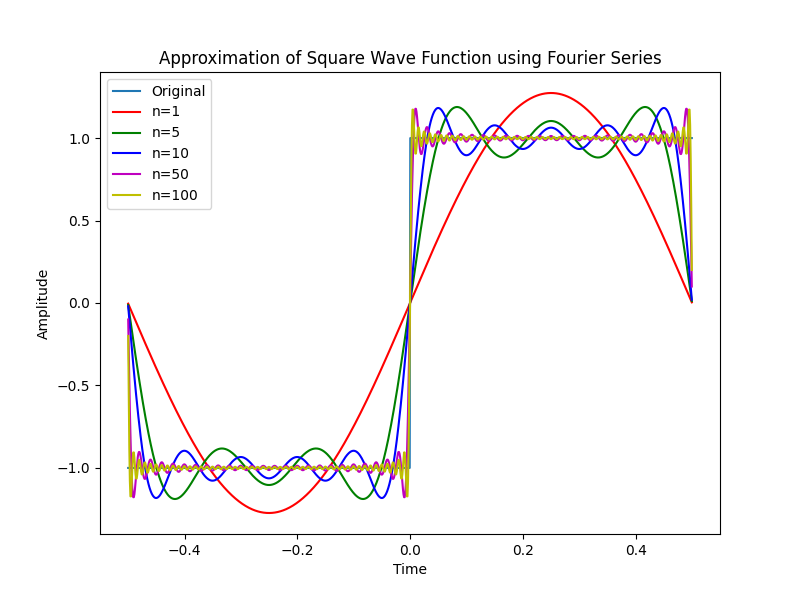
\includegraphics[scale=0.55]{hw3/square_wave.png}}
        \caption{Square Wave Signal Approximation}
        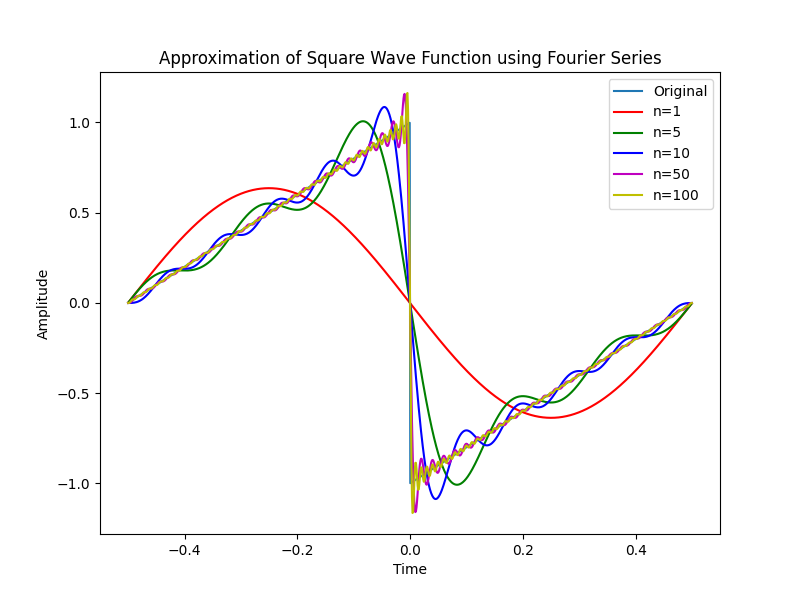
\includegraphics[scale=0.55]{hw3/sawtooth.png}
        \caption{Sawtooth Wave Signal Approximation}
    \end{figure}
\\\\Increasing the number of Fourier Series coefficients (n) has the effect of improving the accuracy of the Fourier Series approximation of a given signal.
\\\\The Fourier Series is a representation of a periodic function as a sum of sinusoidal functions with different amplitudes and frequencies. The more terms (coefficients) we include in the Fourier Series, the more closely the approximation will approximate the original signal.
\\\\In particular, as the number of coefficients increases, the Fourier Series approximation becomes more accurate at representing sharp transitions and irregularities in the signal. This is because higher-order Fourier coefficients correspond to higher-frequency sinusoidal functions, which can capture more complex features of the signal.

\end{enumerate}
\end{document}
